% HiPPO-LegS state as online L^2 projection — TikZ source. Compiles to a tight
% standalone PDF (pdflatex figures/hippo-projection.tex), which
% `book-scaffold build-figures` converts to public/figures/hippo-projection.svg
% (PDF -> SVG via pdftocairo).
%
% The state h(t) is not an ad-hoc memory buffer: it is the coefficient vector of
% the L^2([0,t])-optimal degree-(d_s - 1) polynomial fit to the whole history
% u|_[0,t], expressed in a rescaled Legendre basis g_0, g_1, g_2, .... Maintaining
% these coefficients online, as the window [0,t] grows, is exactly the linear ODE
% h' = -(1/t) A h + (1/t) B u (thm-tf3-hippo-legs).
\documentclass[tikz,border=3pt]{standalone}
\usepackage{amsmath}
\usepackage{amssymb}
\usepackage{tikz}
\usetikzlibrary{positioning,arrows.meta,calc}
\begin{document}
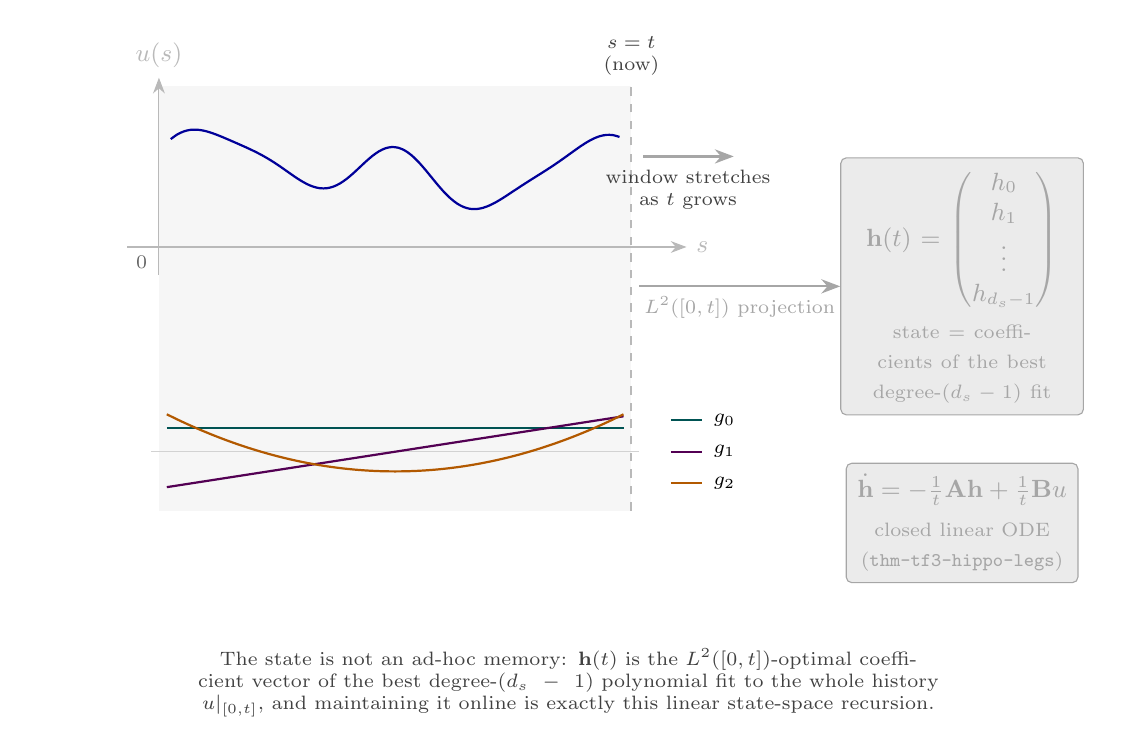
\begin{tikzpicture}[
    font=\small,
    box/.style={draw, gray!70, rounded corners=2pt, align=center,
                minimum height=10mm, inner sep=4pt},
    op/.style={->, >={Stealth[length=2.4mm]}, gray!70, thick},
    axisline/.style={-{Stealth[length=2mm]}, gray!55},
  ]

  % ---------- background: the growing window [0,t], shared by both panels ----------
  \fill[gray!7] (0,-3.35) rectangle (6,2.05);

  % ---------- main panel: signal u(s) on [0,t] ----------
  \draw[axisline] (-0.4,0) -- (6.7,0) node[right, font=\small] {$s$};
  \draw[axisline] (0,-0.35) -- (0,2.15) node[above, font=\small] {$u(s)$};
  \node[font=\scriptsize, text=black!60] at (-0.22,-0.2) {$0$};

  \draw[thick, blue!60!black]
    plot[domain=0.15:5.85, samples=70, smooth]
    (\x,{1.0+0.32*sin(148.97*\x)+0.22*sin(63.03*\x+34.38)+0.10*sin(246.37*\x+68.75)});

  % ---------- shared "now" boundary ----------
  \draw[dashed, gray!55, thick] (6,-3.35) -- (6,2.05);
  \node[above, font=\scriptsize, align=center, text=black!75] at (6,2.05)
    {$s=t$\\(now)};

  % ---------- window advances ----------
  \draw[op] (6.15,1.15) -- (7.3,1.15);
  \node[below, font=\scriptsize, align=center, text=black!75] at (6.72,1.1)
    {window stretches\\as $t$ grows};

  % ---------- basis panel: rescaled Legendre g_0, g_1, g_2 on the same window ----------
  \draw[gray!35] (-0.1,-2.6) -- (6.1,-2.6);
  \draw[thick, teal!65!black] (0.1,-2.30) -- (5.9,-2.30);
  \draw[thick, violet!65!black] (0.1,-3.05) -- (5.9,-2.15);
  \draw[thick, orange!70!black]
    plot[domain=0.1:5.9, samples=40, smooth] (\x,{-2.85+0.0862*(\x-3)^2});

  \draw[teal!65!black, thick] (6.5,-2.2) -- (6.9,-2.2);
  \node[right, font=\scriptsize] at (6.92,-2.2) {$g_0$};
  \draw[violet!65!black, thick] (6.5,-2.6) -- (6.9,-2.6);
  \node[right, font=\scriptsize] at (6.92,-2.6) {$g_1$};
  \draw[orange!70!black, thick] (6.5,-3.0) -- (6.9,-3.0);
  \node[right, font=\scriptsize] at (6.92,-3.0) {$g_2$};

  % ---------- projection arrow + state vector + dynamics ----------
  \node[box, fill=black!8, minimum width=26mm, text width=28mm] (hbox) at (10.2,-0.5)
    {$\mathbf h(t)=\begin{pmatrix} h_0\\ h_1\\ \vdots\\ h_{d_s-1}\end{pmatrix}$\\[4pt]
     \scriptsize state = coefficients of the best degree-$(d_s-1)$ fit};
  \draw[op] (6.1,-0.5) -- (hbox.west)
    node[midway, below, font=\scriptsize, align=center] {$L^2([0,t])$ projection};

  \node[box, fill=black!8, below=6mm of hbox] (dynbox)
    {$\dot{\mathbf h} = -\tfrac{1}{t}\mathbf A\mathbf h + \tfrac{1}{t}\mathbf B u$\\[3pt]
     \scriptsize closed linear ODE\\
     \scriptsize (\texttt{thm-tf3-hippo-legs})};

  % ---------- bottom caption: y tracks dynbox's true height, x recentred on figure ----------
  \node[align=center, text width=13.5cm, font=\scriptsize, text=black!75,
        below=7mm of dynbox, xshift=-5.0cm]
    {The state is not an ad-hoc memory: $\mathbf h(t)$ is the $L^2([0,t])$-optimal
     coefficient vector of the best degree-$(d_s-1)$ polynomial fit to the whole
     history $u|_{[0,t]}$, and maintaining it online is exactly this linear
     state-space recursion.};

\end{tikzpicture}
\end{document}
